\documentclass{beamer}
\usetheme{Madrid}
\usecolortheme{default}


\usepackage[T1]{fontenc}
\usepackage[utf8]{inputenc}
\usepackage{amsmath,amssymb,bm,mathtools}
\usepackage{xcolor}
\usepackage{hyperref}
\usepackage{microtype}

\graphicspath{{./figures/}}
\usepackage{booktabs}


\title[Project 1]{Project 1}
\subtitle{CS 332, Fall 2025}
\author{Ben Cole \and Koshi Harashima\\ Northwestern University}
\date{8 October, 2025}


\begin{document}

\maketitle

\begin{frame}{Outline}
  \tableofcontents
\end{frame}

\AtBeginSection[]{
  \begin{frame}{Outline}
    \tableofcontents[currentsection]
  \end{frame}
}

\section{Part 1}


% Slide 2 Introductio 1: Executive Summary
\begin{frame}{Part 1}
In Part 1, 
\medskip
\begin{itemize}
  \item \textbf{Methods:} Exact Estimation and Monte Carlo Estimation.
  \item \textbf{Results:} Koshi's strategy did not work well, while Ben's strategy worked pretty well.
  \item \textbf{Takeaways:}: Monte Carlo approximately becomes exact as the sample size increases. The better bid strategy is to bid conservatively.
\end{itemize}
\end{frame}


% Slide 3 Modeliing
\begin{frame}{Model}
\medskip
\begin{itemize}
  \item \textbf{Setting:} single-item, first-price, two bidders (you vs.\ one opponent).
  \item \textbf{Private value:} $v\in\{10,20,\dots,100\}$. You bid $b\in[0,v]$.
  \item \textbf{Payoff:} if win, $u=v-b$; else $u=0$.
  \item \textbf{Winning probability:}
    \[
      P_{\text{win}}(b)=P(\text{opp}<b)+\tfrac12P(\text{opp}=b).
    \]
  \item \textbf{Objective:}
    \[
      EU(v,b)=(v-b)\,P_{\text{win}}(b),\qquad b^*(v)=\arg\max_{0\le b\le v}EU(v,b).
    \]
  \item MC = Monte Carlo,\; EU = Expected Utility,\; opt = optimal.
\end{itemize}
\end{frame}


% Slide4: Calculation methods 
\subsection{1. winning probability and expected utility with your bids}
\begin{frame}{Calculation methods: Exact \; vs \; Monte Carlo}
\medskip
\begin{itemize}
  \item \textbf{Empirical analysis:}\\
  pick $V\sim\mathrm{Unif}\{10,\dots,100\}$; sample opponent bid set $\{b_i\}_{i=1}^n$ for that $V$.
  \item \textbf{Exact estimate:}\\
    {\centering
    \[
    \widehat{P}_{\mathrm{win}}(b)
    \;=\;\frac{\#\{b_i < b\} \;+\; \tfrac{1}{2}\#\{b_i = b\}}{n}
    \]
    \[
    \mathrm{EU}_{\mathrm{exact}}(v,b)
    \;=\; (v - b)\,\widehat{P}_{\mathrm{win}}(b)
    \]}
  \item \textbf{Monte Carlo estimator:} \\
  draw $B_{\text{opp}}^{(t)}$ from empirical model for $t=1,\dots,T$,
    \[
      \widehat{EU}_{\text{MC}}(v,b)=\frac{1}{T}\sum_{t}\Big(\mathbf{1}\{b>B_{\text{opp}}^{(t)}\}+\tfrac12\mathbf{1}\{b=B_{\text{opp}}^{(t)}\}\Big)(v-b).
    \]
    \begin{itemize}
        \item use $T=20{,}000$ for stable MC estimates.
    \end{itemize}
\end{itemize}
\end{frame}


% Result - koshi - 
\begin{frame}{Koshi's Case}
1.Calculate your winning probability and expected utility with your bids submitted in Ex 1.2 for each of your values.
\begin{center}
\small
\begin{tabular}{@{}rrrrrrrr@{}}
\toprule
value & my bid & win prob & EU exact & EU MC & opt bid & opt EU & regret \\
\midrule
 10 &   9 & 0.091 & 0.091 & 0.088 &  5 & 0.334 & 0.243 \\
 20 &  19 & 0.252 & 0.252 & 0.250 & 11 & 1.740 & 1.487 \\
 30 &  29 & 0.418 & 0.418 & 0.417 & 11 & 3.694 & 3.276 \\
 40 &  39 & 0.577 & 0.577 & 0.580 & 21 & 6.529 & 5.952 \\
 50 &  49 & 0.716 & 0.716 & 0.718 & 21 & 9.984 & 9.268 \\
 60 &  59 & 0.805 & 0.805 & 0.806 & 31 &14.713 &13.908 \\
 70 &  69 & 0.855 & 0.855 & 0.856 & 31 &19.804 &18.949 \\
 80 &  79 & 0.905 & 0.905 & 0.904 & 41 &25.462 &24.557 \\
 90 &  89 & 0.950 & 0.950 & 0.951 & 41 &32.007 &31.057 \\
100 &  99 & 0.991 & 0.991 & 0.991 & 51 &38.675 &37.685 \\
\bottomrule
\end{tabular}
\end{center}
I took a strategy in which I always bid \(b=v-1\) (one unit below valuation).
Average Regret : \textbf{14.63}
\end{frame}


% Result - Ben -
\begin{frame}{Ben's Case}
2. Calculate your winning probability and expected utility with your bids submitted in Ex 1.2 for each of your values.
\begin{center}
\small
\begin{tabular}{@{}rrrrrrrr@{}}
\toprule
value & my bid & win prob & EU exact & EU MC & opt bid & opt EU & regret \\
\midrule
 10 &   9 & 0.091 & 0.091 & 0.088 &  5 & 0.334 & 0.243 \\
 20 &  15 & 0.216 & 1.080 & 1.075 & 11 & 1.740 & 0.660 \\
 30 &  20 & 0.291 & 2.909 & 2.865 & 11 & 3.694 & 0.785 \\
 40 &  25 & 0.375 & 5.625 & 5.569 & 21 & 6.529 & 0.904 \\
 50 &  30 & 0.455 & 9.091 & 9.089 & 21 & 9.984 & 0.893 \\
 60 &  30 & 0.455 &13.636 &13.633 & 31 &14.713 & 1.076 \\
 70 &  35 & 0.532 &18.614 &18.648 & 31 &19.804 & 1.190 \\
 80 &  40 & 0.607 &24.273 &24.406 & 41 &25.462 & 1.189 \\
 90 &  45 & 0.677 &30.477 &30.651 & 41 &32.007 & 1.530 \\
100 &  50 & 0.745 &37.273 &37.403 & 51 &38.675 & 1.403 \\
\bottomrule
\end{tabular}
\end{center}
Average Regret : \textbf{0.98}
\end{frame}

% Slide 7 rest of Part 1
\subsection{2. the optimal bids}
\begin{frame}{Optimal-Bids}
\begin{itemize}
    \item Calculate the optimal bids values.
    \[b^{*}(v)=\arg\max_{0\le b\le v}\; (v - b)\,F(b)\]
    \begin{itemize}
        \item the answer is 
    \end{itemize} 
        {\small
        \begin{center}
        \begin{tabular}{@{}rrrrrrrr@{}}
        \toprule
        value & b\_opt\_exact & util\_opt\_exact & b\_opt\_mc & util\_opt\_mc \\
        \midrule
        10  &  5.1 &  0.3341 &  1.6 &  0.3507 \\
        20  & 11.1 &  1.7395 & 11.1 &  1.8067 \\
        30  & 11.1 &  3.6941 & 11.1 &  3.8367 \\
        40  & 21.1 &  6.5291 & 21.6 &  6.6608 \\
        50  & 21.1 &  9.9836 & 21.6 & 10.2808 \\
        60  & 31.1 & 14.7127 & 31.3 & 14.9455 \\
        70  & 31.1 & 19.8036 & 31.3 & 20.1530 \\
        80  & 41.1 & 25.4618 & 41.0 & 25.8814 \\
        90  & 41.1 & 32.0073 & 41.0 & 32.5176 \\
        100 & 51.1 & 38.6755 & 41.0 & 39.1539 \\
        \bottomrule
        \end{tabular}
        \end{center}}
\end{itemize}
\end{frame}

\subsection{3. Better bid strategy}
\begin{frame}{About Good Strategy}
\begin{itemize}
    \item Compare the utility you obtained to the optimal utility you could have obtained.  Can you conclude anything about a good strategy in this auction?
    \begin{itemize}
        \item from Koshi's case: we observe that it is not recommended to bid too close to your valuation.
        \item From Ben's case: he bids conservatively, yet his bids are close to the optimal bids and show very good expected-utility performance.
        \end{itemize}
\end{itemize}
\vspace{0.5em}
\begin{columns}[t]
  \begin{column}{0.48\textwidth}
    \centering
    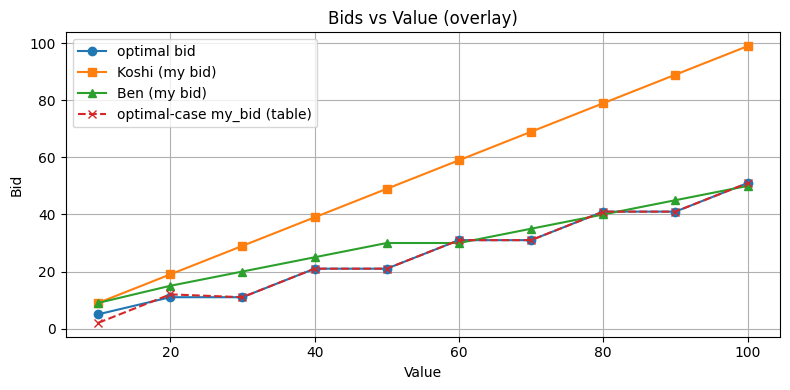
\includegraphics[width=\linewidth]{332Project1/figures/bid.png}
    \vspace{0.4em}
    {\footnotesize (a) Bid vs.\ value}
  \end{column}
  \begin{column}{0.48\textwidth}
    \centering
    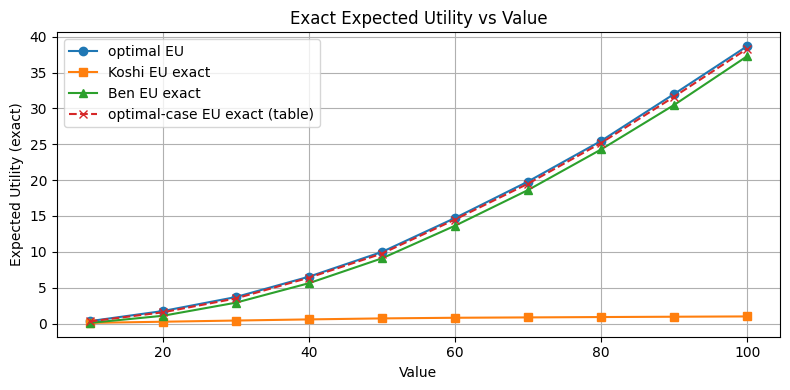
\includegraphics[width=\linewidth]{332Project1/figures/utility.png}
    \vspace{0.4em}
    {\footnotesize (b) Expected utility vs.\ value}
  \end{column}
\end{columns}
\end{frame}

\begin{frame}{Appendix: Regret}
    \begin{figure}
        \centering
        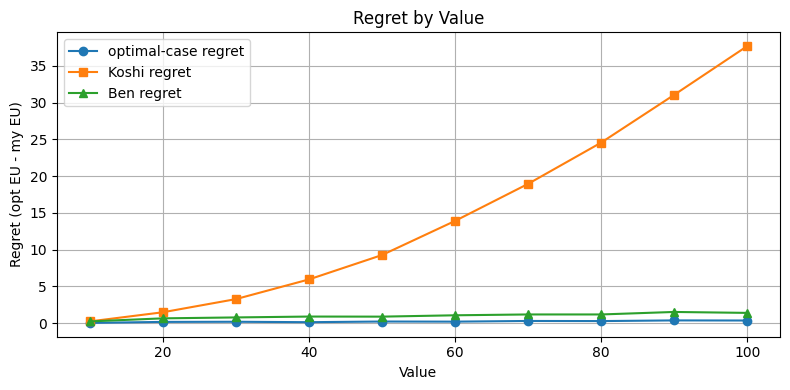
\includegraphics[width=1\linewidth]{332Project1/figures/regret.png}
    \vspace{0.4em}
    {\footnotesize (c) Regret}
    \end{figure}
\end{frame}

\section{Part 2}

\begin{frame}{Part 2}
    In Part 2, we consider two things; 
    \medskip
    \begin{itemize}
        \item optimal data-driven bid strategy, 
        \item The theoretically optimal bid in a two-player auction.
    \end{itemize}
\end{frame}

\subsection{optimal data-driven bid strategy}
% --- Slide 1: Goal & Method ---
\begin{frame}{Method}
\small
\textbf{Goal.} Choose a bid function $b(v)$ to maximize expected profit:
\[
b^*(v)=\arg\max_{0\le b\le v}(v-b)\,\Pr(B_{\text{opp}}\le b\mid v).
\]
\textbf{What we estimate.} The win-probability CDF at value $v$:
\[
F_v(b)=\Pr(B_{\text{opp}}\le b\mid v).
\]
\textbf{How we estimate (from \texttt{bid\_data.csv}).} Empirical CDF:
\[
\hat F_v(b)=\frac{1}{n_v}\sum_{i=1}^{n_v}\mathbf{1}\{b_i\le b\}.
\]
\textbf{Plug-in rule.}
\[
\hat b^*(v)=\arg\max_{0\le b\le v}(v-b)\,\hat F_v(b).
\]
\end{frame}

\begin{frame}{Empirical CDF}
\begin{columns}[T,onlytextwidth]
  \column{0.33\textwidth}
  \begin{figure}
    \centering
    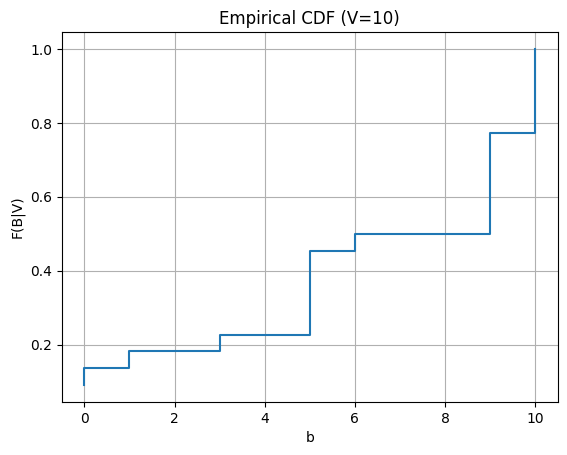
\includegraphics[width=\linewidth]{332Project1/figures/v=10.png}
    \caption{V=10}\label{fig:v10}
  \end{figure}

  \column{0.33\textwidth}
  \begin{figure}
    \centering
    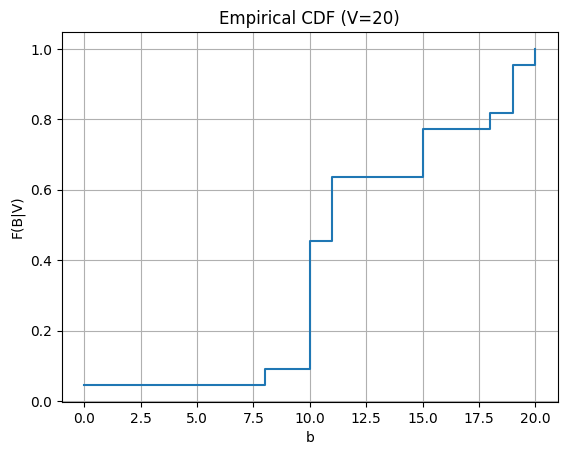
\includegraphics[width=\linewidth]{332Project1/figures/v=20.png}
    \caption{V=20}\label{fig:v20}
  \end{figure}

  \column{0.33\textwidth}
  \begin{figure}
    \centering
    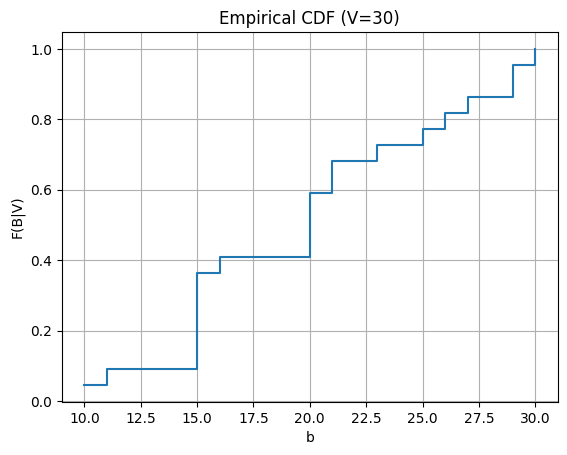
\includegraphics[width=\linewidth]{332Project1/figures/v=30.png}
    \caption{V=30}\label{fig:v30}
  \end{figure}
\end{columns}
\end{frame}


\begin{frame}{Appendix: Distribution}
    \begin{figure}
        \centering
        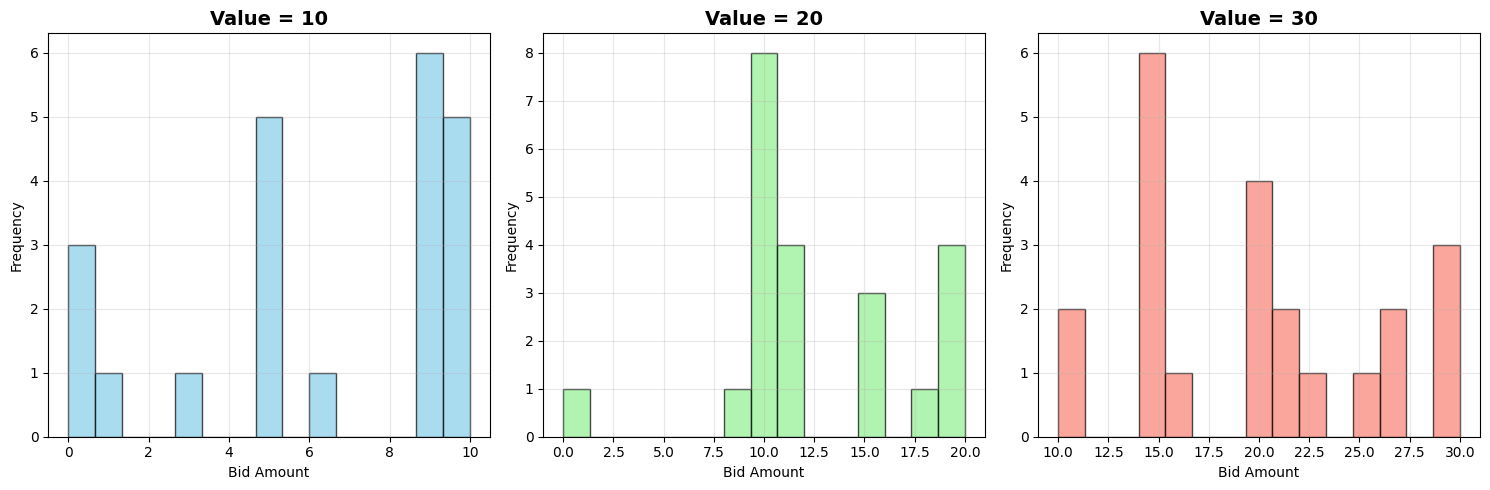
\includegraphics[width=0.7\linewidth]{332Project1/figures/barplot.png}
        \caption{Discrete Distribution}
        \label{fig:placeholder}
    \end{figure}
    \begin{figure}
        \centering
        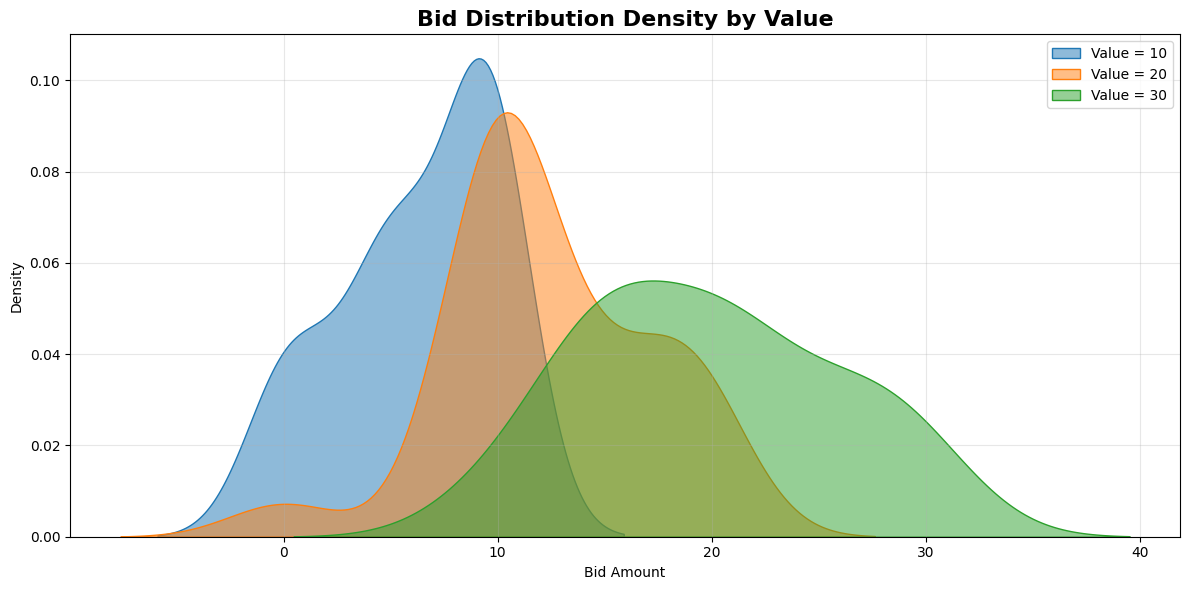
\includegraphics[width=0.5\linewidth]{332Project1/figures/Distribution.png}
        \caption{Continuous Distribution}
        \label{fig:placeholder}
    \end{figure}
\end{frame}

\begin{frame}{Conclusion}
\small
\textbf{Message.} As $n$ increases, the empirical win CDF $\hat F_v$ approaches the true $F_v$, so the plug-in bid converges to the optimum:
\[
\hat b^*(v)=\arg\max_{0\le b\le v} (v-b)\,\hat F_v(b)
\;\longrightarrow\;
b^*(v).
\]
\textbf{Estimator.}
\[
\hat F_v(b)=\frac{1}{n_v}\sum_{i=1}^{n_v}\mathbf{1}\{b_i\le b\}.
\]
\end{frame}


\subsection{optimal bid in theory}

\begin{frame}{Observation}
\small
\begin{itemize}
  \item \textbf{Second-price:} Truthful bidding (bid = value) is a dominant strategy (referred in class).
  \item \textbf{First-price:} : It seems like the optimal bid is linear in value, but its coefficient is half not 1.\\
  \item \textbf{Optimal-bid in First-price auction}\\
  Optimal bid problem is formulated by following formula;
    \[  
        b^{*}=\arg\max_{b}\,(v-b)\,\Pr(\text{win at } b).
    \]
\end{itemize}
\begin{figure}
    \centering
    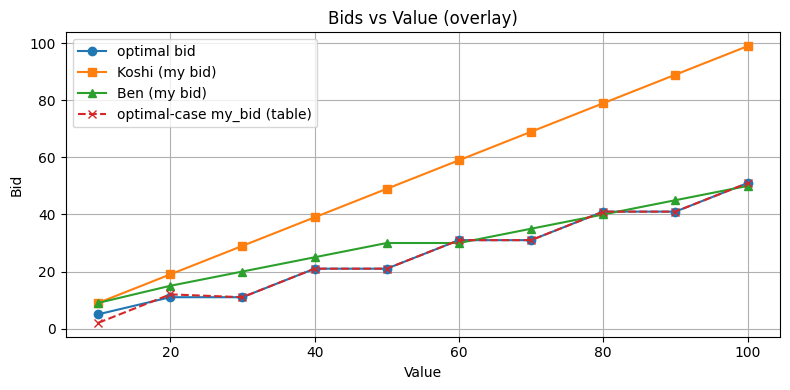
\includegraphics[width=0.5\linewidth]{332Project1/figures/bid.png}
    \caption{bid strategy}
    \label{fig:placeholder}
\end{figure}
\end{frame}

\begin{frame}{Bid Strategy in First-Price Auction}
\small
\textbf{Setup:} Two bidders, values i.i.d.\ $U[0,1]$.\\
\begin{itemize}
    \item Suppose opponent's bid strategy is linear in his value.
    \item Considering Best respond to a opponent whose bid strategy is $b(x)=\alpha x$
\end{itemize}
\[
\Pr(\text{win at bid }b)=\Pr(\alpha X<b)=\tfrac{b}{\alpha}
\]
so, 
\[
b^{*}=\arg\max_{b}(v-b)\tfrac{b}{\alpha} (= U).
\]
FOC in b:\\
\[
\partial U/\partial b=\tfrac{1}{\alpha}(v-2b)=0 \;\ \Rightarrow\; b^*(v)=\tfrac12 v.
\]
By symmetry, 
\[
b(v)=\alpha v=b^*(v) \ \Rightarrow\; \alpha=\tfrac12.
\]

\end{frame}

\begin{frame}{Usage of AI}
    AI was used for figures, code, and design; final review and responsibility by the authors.
\end{frame}

\end{document}
